% $Id: template.tex 11 2007-04-03 22:25:53Z jpeltier $

\documentclass{vgtc}                          % final (conference style)
%\documentclass[review]{vgtc}                 % review
%\documentclass[widereview]{vgtc}             % wide-spaced review
%\documentclass[preprint]{vgtc}               % preprint
%\documentclass[electronic]{vgtc}             % electronic version

%% Uncomment one of the lines above depending on where your paper is
%% in the conference process. ``review'' and ``widereview'' are for review
%% submission, ``preprint'' is for pre-publication, and the final version
%% doesn't use a specific qualifier. Further, ``electronic'' includes
%% hyperreferences for more convenient online viewing.

%% Please use one of the ``review'' options in combination with the
%% assigned online id (see below) ONLY if your paper uses a double blind
%% review process. Some conferences, like IEEE Vis and InfoVis, have NOT
%% in the past.

%% Figures should be in CMYK or Grey scale format, otherwise, colour 
%% shifting may occur during the printing process.

%% These few lines make a distinction between latex and pdflatex calls and they
%% bring in essential packages for graphics and font handling.
%% Note that due to the \DeclareGraphicsExtensions{} call it is no longer necessary
%% to provide the the path and extension of a graphics file:
%% \includegraphics{diamondrule} is completely sufficient.
%%
\ifpdf%                                % if we use pdflatex
  \pdfoutput=1\relax                   % create PDFs from pdfLaTeX
  \pdfcompresslevel=9                  % PDF Compression
  \pdfoptionpdfminorversion=7          % create PDF 1.7
  \ExecuteOptions{pdftex}
  \usepackage{graphicx}                % allow us to embed graphics files
  \DeclareGraphicsExtensions{.pdf,.png,.jpg,.jpeg} % for pdflatex we expect .pdf, .png, or .jpg files
\else%                                 % else we use pure latex
  \ExecuteOptions{dvips}
  \usepackage{graphicx}                % allow us to embed graphics files
  \DeclareGraphicsExtensions{.eps}     % for pure latex we expect eps files
\fi%

%% it is recomended to use ``\autoref{sec:bla}'' instead of ``Fig.~\ref{sec:bla}''
\graphicspath{{figures/}{pictures/}{images/}{./}} % where to search for the images

\usepackage{microtype}                 % use micro-typography (slightly more compact, better to read)
\PassOptionsToPackage{warn}{textcomp}  % to address font issues with \textrightarrow
\usepackage{textcomp}                  % use better special symbols
\usepackage{mathptmx}                  % use matching math font
\usepackage{times}                     % we use Times as the main font
\renewcommand*\ttdefault{txtt}         % a nicer typewriter font
\usepackage{cite}                      % needed to automatically sort the references
\usepackage{tabu}                      % only used for the table example
\usepackage{booktabs}                  % only used for the table example
%% We encourage the use of mathptmx for consistent usage of times font
%% throughout the proceedings. However, if you encounter conflicts
%% with other math-related packages, you may want to disable it.


%% If you are submitting a paper to a conference for review with a double
%% blind reviewing process, please replace the value ``0'' below with your
%% OnlineID. Otherwise, you may safely leave it at ``0''.
\onlineid{0}

%% declare the category of your paper, only shown in review mode
\vgtccategory{Research}

%% allow for this line if you want the electronic option to work properly
\vgtcinsertpkg

%% In preprint mode you may define your own headline.
%\preprinttext{To appear in an IEEE VGTC sponsored conference.}


%MC Stuff
\usepackage{subcaption}

%% Paper title.

\title{Black Hat Visualization}

%% This is how authors are specified in the conference style

%% Author and Affiliation (single author).
%%\author{Roy G. Biv\thanks{e-mail: roy.g.biv@aol.com}}
%%\affiliation{\scriptsize Allied Widgets Research}

%% Author and Affiliation (multiple authors with single affiliations).
%%\author{Roy G. Biv\thanks{e-mail: roy.g.biv@aol.com} %
%%\and Ed Grimley\thanks{e-mail:ed.grimley@aol.com} %
%%\and Martha Stewart\thanks{e-mail:martha.stewart@marthastewart.com}}
%%\affiliation{\scriptsize Martha Stewart Enterprises \\ Microsoft Research}

%% Author and Affiliation (multiple authors with multiple affiliations)
\author{Michael Correll\\ %
        \scriptsize University of Washington %
\and Jeffrey Heer\\ %
     \scriptsize University of Washington %
}

%% A teaser figure can be included as follows, but is not recommended since
%% the space is now taken up by a full width abstract.
\teaser{
	\centering
	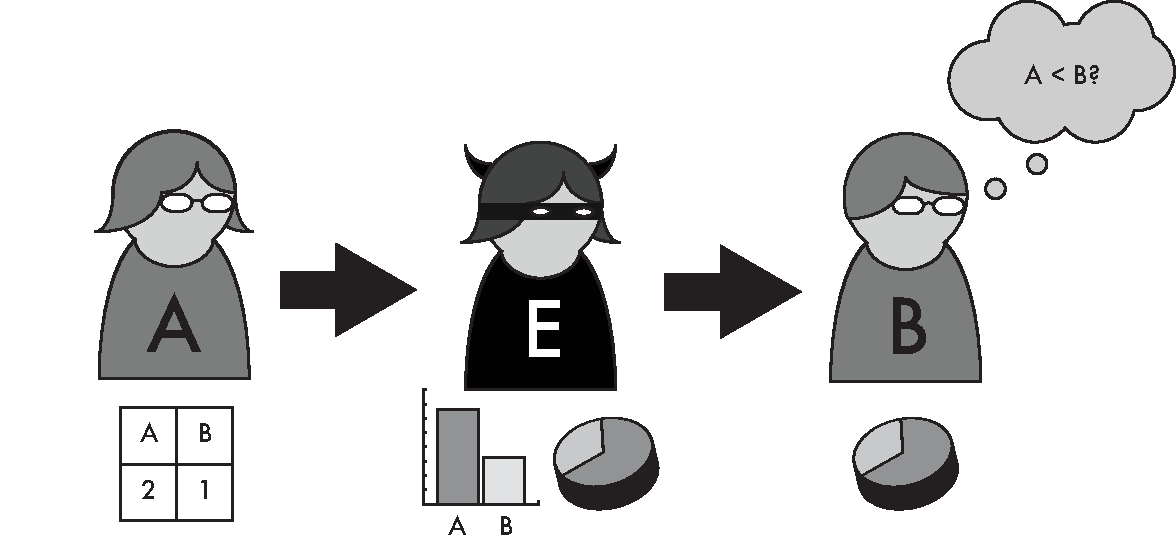
\includegraphics[width=0.4\textwidth]{/pictures/model.pdf}
  \caption{A model of a visualization ``attack.'' Data scientist \textbf{A}lex has a dataset they wish to communicate to stakeholder \textbf{B}rook. Unfortunately, Alex must go through visualization designer \textbf{E}rin, who has malicious intent. Erin has many potential visualization designs at their disposal, but chooses one that is likely to cause Brook to have an incorrect impression of the data. }
  \label{fig:teaser}
}

%% Abstract section.
\abstract{
	People lie, mislead, and bullshit in a myriad of ways. Visualizations, as a form of communication, are no exception to these tendencies. Yet, the language we use to describe how people can use visualizations to mislead can be relatively sparse. For instance, one can be ``lying with vis'' or using ``deceptive visualizations.'' In this paper, we use the language of computer security to expand the space of ways that unscrupulous people (black hats) can manipulate visualizations for nefarious ends. In addition to forms of deception well-covered in the visualization literature, we also focus on visualizations which have fidelity to the underlying data (and so may not be considered deceptive in the ordinary use of the term in visualization), but still have negative impact on how data are perceived. We encourage designers to think defensively and comprehensively about how their visual designs can result in data being misinterpreted.
} % end of abstract

%% ACM Computing Classification System (CCS). 
%% See <http://www.acm.org/class/1998/> for details.
%% The ``\CCScat'' command takes four arguments.

\CCScatlist{ 
  \CCScat{K.7.m}{The Computing Profession}{Miscellaneous}{Ethics}
}

%% Copyright space is enabled by default as required by guidelines.
%% It is disabled by the 'review' option or via the following command:
% \nocopyrightspace

%%%%%%%%%%%%%%%%%%%%%%%%%%%%%%%%%%%%%%%%%%%%%%%%%%%%%%%%%%%%%%%%
%%%%%%%%%%%%%%%%%%%%%% START OF THE PAPER %%%%%%%%%%%%%%%%%%%%%%
%%%%%%%%%%%%%%%%%%%%%%%%%%%%%%%%%%%%%%%%%%%%%%%%%%%%%%%%%%%%%%%%%

\begin{document}

%% The ``\maketitle'' command must be the first command after the
%% ``\begin{document}'' command. It prepares and prints the title block.

%% the only exception to this rule is the \firstsection command
\firstsection{Introduction}

\maketitle

%% \section{Introduction} %for journal use above \firstsection{..} instead
Designers of visualizations have a great deal of power over how data are interpreted. Ideally, designers are interested in accurately presenting data in order to foster responsible and evidence-based decision-making. In the real world, however, designers may have more nefarious goals. In these situations, designers can use visualizations as an \emph{attack vector} to distort how an audience perceives and uses data. We refer to this strategy of altering visualization designs to encourage specific interpretations as ``black hat vis.'' In prior work in the visualization community, many of these black hat techniques are said to generate ``deceptive'' visualization, or ``vis lies''~\cite{vislies2016}. This language conflates \emph{poor} visualization design and \emph{malicious} visualization design. The binary notion that a visualization is either deceptive or not also elides the subtlety of some of these techniques, which may have an impact on how data are perceived and used without altering the fidelity with which they are presented.
 
There is extensive prior work on how visualizations can be deceptive, including empirical studies on the efficacy of these deceptions~\cite{pandey2015deceptive}. However, discussions of deceptive visualizations can be ad hoc, built around a limited set of examples. Compared to the rich variety of ways that humans can and have deceived each other (and themselves), visualization has a relatively sparse set of examples of deceptive practices. There are a set of standard examples that are repeated frequently  (Fig.~\ref{fig:examples}), giving the impression that deceptive visualizations are the uncommon product of a small set of bad apples. It is our contention that a) the intent to persuade (and, so, potentially, to deceive) is ubiquitous in visualization, and b) the space of known deceptive techniques ought to be expanded to match this ubiquity.

In order to provide an initial framework for expanding the space of deceptive techniques in visualization, we borrow terminology from computer security. In security, ``black hats'' are attackers with malicious or destructive intent. Visualization designers, as intermediaries between a data set (to which a stakeholder may or may not have direct access) and a wider audience, are well-situated to perform ``man in the middle'' attacks (Fig.~\ref{fig:teaser}). \textbf{Black Hat Visualization} is the blanket term we use to describe all of the actions that malicious visualization designers can take to meet their goals. Creating outright ``lying'' visualizations is just one small category in this larger space of bad behavior. In this paper, we lay out some of the other forms these attacks can take, under the principle that a good defense requires a comprehensive threat analysis. In particular, we focus on four categories of attacks---intentional breaks of convention, data manipulation, obfuscation, and nudging---as examples of more comprehensive ways that visualizations can be used with ill intent. In some cases, these attacks can happen by chance or inexperience. However, if we can defend against the evil, then we can also defend against the incompetent.

\begin{figure*}
	\centering
	\begin{subfigure}{0.45\columnwidth}
		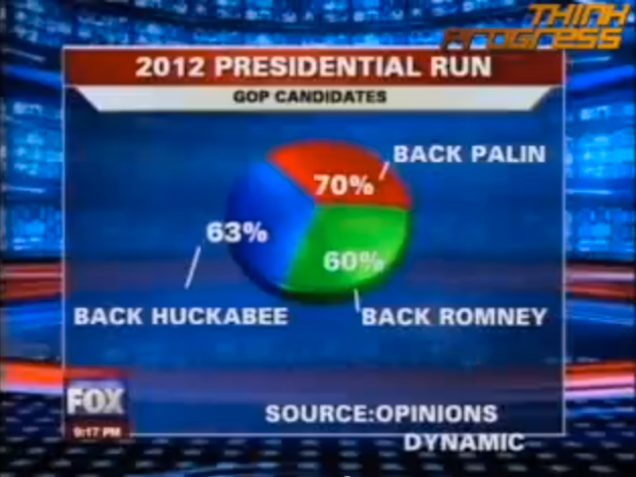
\includegraphics[width=\textwidth]{pictures/foxpie.png}
		\caption{A ``lying'' pie chart}
		\label{fig:badpie}
	\end{subfigure}
	~
	\begin{subfigure}{0.45\columnwidth}
		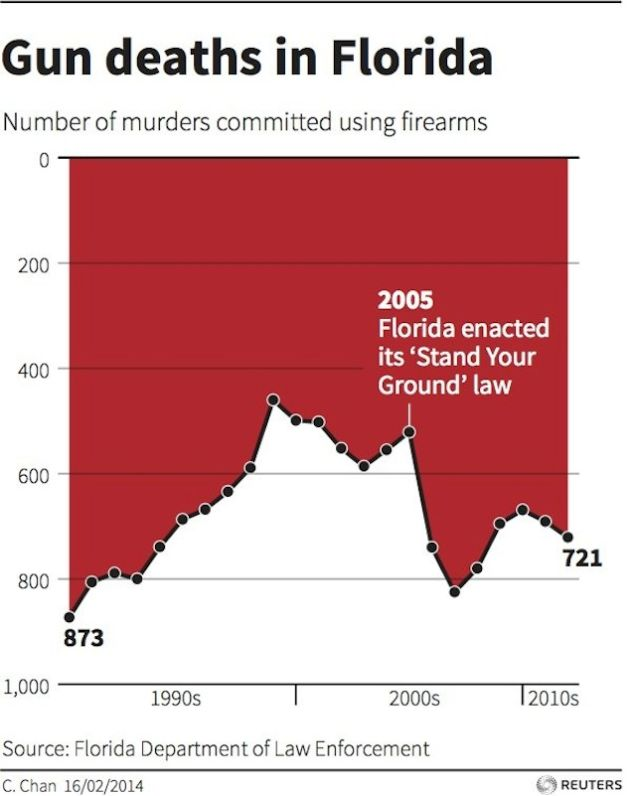
\includegraphics[width=\textwidth]{pictures/gundeaths.jpg}
		\caption{A ``lying'' line graph}
	\end{subfigure}
    ~
	\begin{subfigure}{0.45\columnwidth}
		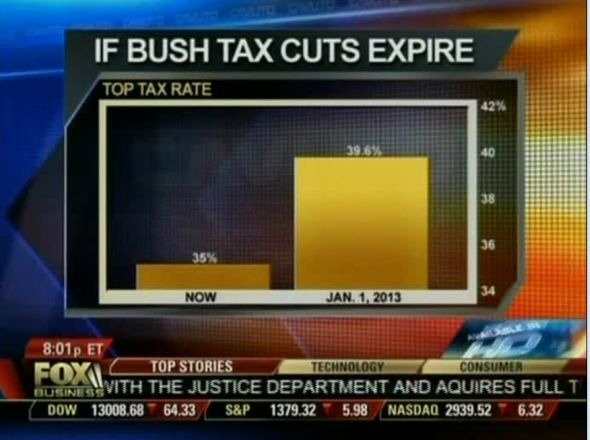
\includegraphics[width=\textwidth]{pictures/foxbar.jpg}
		\caption{A ``lying'' bar chart}
		\label{fig:badbar}
	\end{subfigure}
	\caption{Examples of lying visualizations that are nearly ubiquitous in the discussion of deceptive visualizations. A reverse Google image search reveals millions of hits for each visualization, used in sites with titles ranging from ``\href{https://blog.heapanalytics.com/how-to-lie-with-data-visualization/}{How to Lie with Data Visualization}'' to ``\href{http://www.visualnews.com/2015/11/06/6-data-visualizations-that-failed-at-life/}{6 Data Visualizations That Failed at Life}.'' }
	\label{fig:examples}
\end{figure*}

\section{Broken Conventions}

The interpretation of visualizations is an acquired ability, and this ability is neither monolithic nor universal \cite{boy2014principled}. For instance, a Pew Research poll on scientific knowledge found that only 63\% of Americans could correctly interpret the trends in a scatterplot~\cite{pew2015}. For those with graphical literacy, a great deal of the information in a chart is conveyed \emph{implicitly}, through the conventions of the medium~\cite{kennedy2016work}. For instance, we expect a pie chart to convey a part/whole relationships, and thus for its components to add up to 100\%, and are surprised when the components do not (as in Fig.~\ref{fig:badpie}). We expect that the heights of bars in a bar chart are proportional to their value; truncated y-axes defy this expectation (as in Fig.~\ref{fig:badbar}). People who predominantly write left-to-right expect time to mapped from left to right on the x-axis~\cite{bergen2012writing,tversky1991cross}, and so on. By defying these implicit conventions, an attacker can create a visualization which is technically ``correct'' (in that it is a valid and straightforward mapping from data to mark), but still misleads.

\begin{figure}
	\centering
	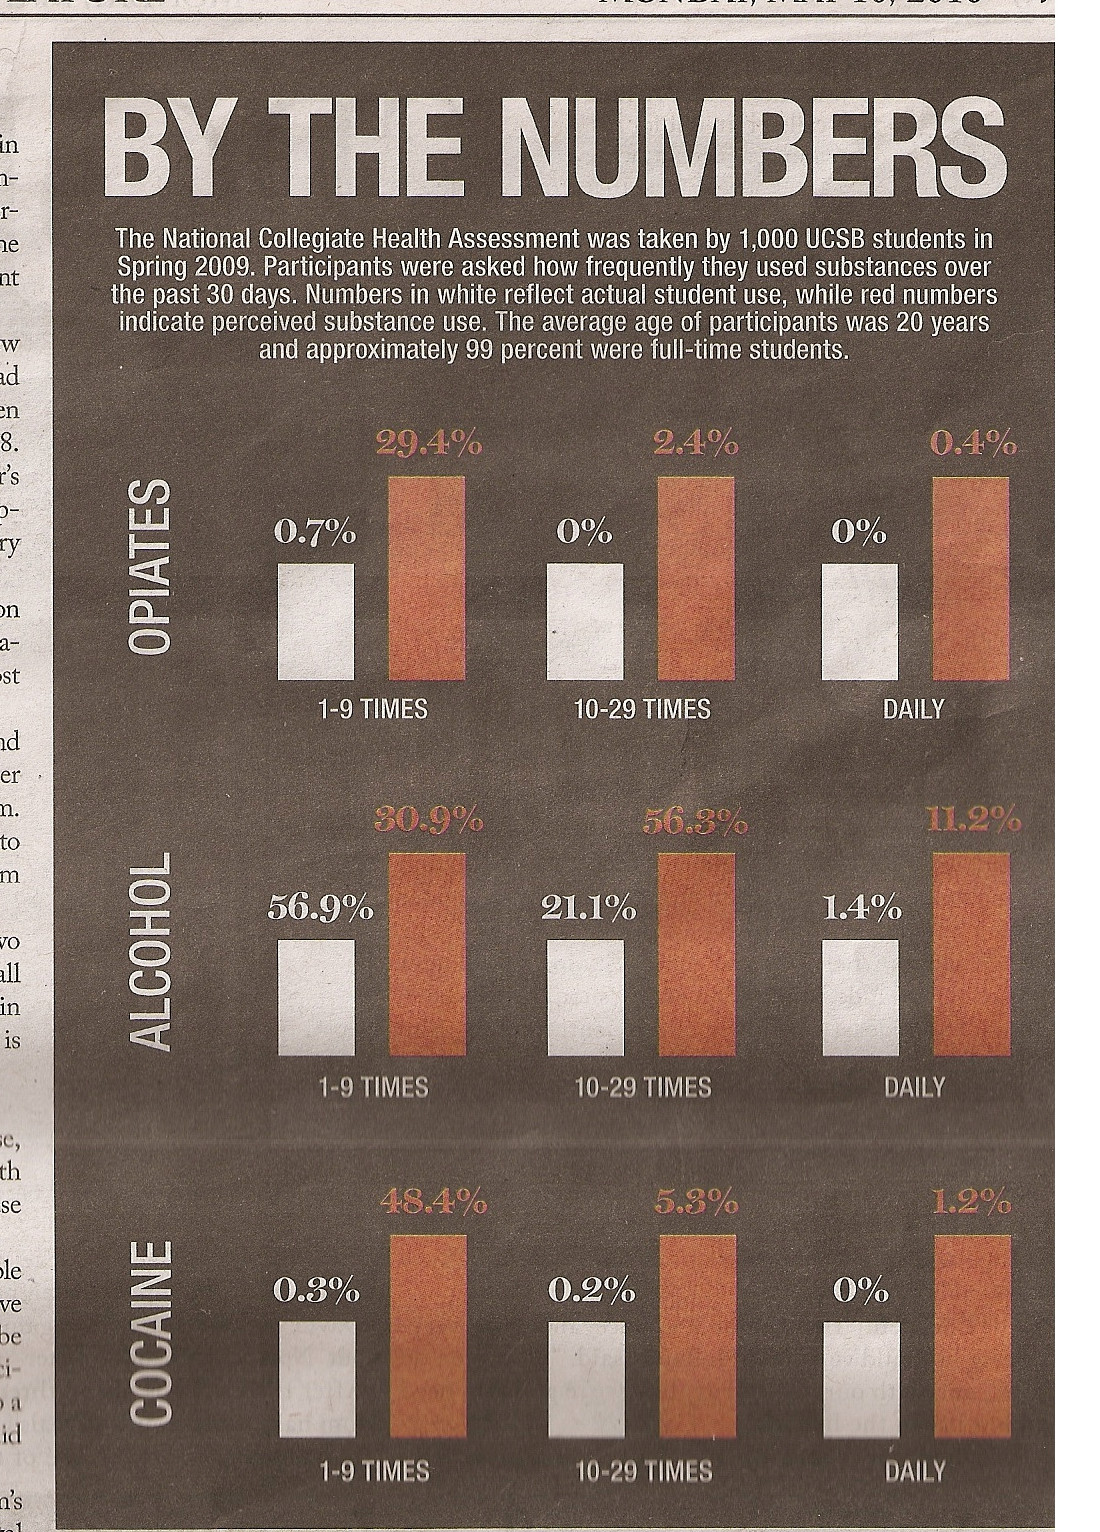
\includegraphics[width=.8\columnwidth]{pictures/badbars.jpg}
	\caption{A set of non sequitur bar charts~\cite{eagereyes}. The visualization follows the visual conventions of bar charts, but there is no connection between the data values and the height of the bars.}
	\label{fig:nonseq}
\end{figure}

Another form of attack that piggybacks on established visual conventions is to have no relation between data and mark (as in Fig.~\ref{fig:nonseq}). In the wild, many charts and graphs are simply conceived of as ``number decoration''\cite{moritz2017}. Charts are frequently associated with scientific evidence and other trustworthy sources of information. Charts can therefore be persuasive even if they are superfluous or uninformative~\cite{tal2016blinded}. A black hat designer can take advantage of this fact by choosing not to directly visualize data that may be contrary to their intended goals, but instead representing it with ``non sequitur'' visualizations. A non sequitur visualization could consist of ``decorative'' bar charts or pie charts with arbitrary values, and the actual (unfavorable) data values represented textually elsewhere.

\section{Data Manipulation}

\begin{figure}
	\centering
	\begin{subfigure}{0.85\columnwidth}
		\centering
		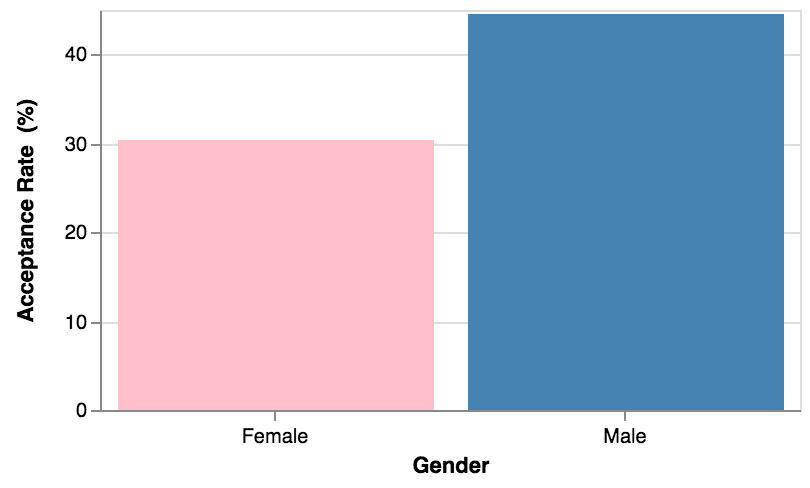
\includegraphics[width=.45\columnwidth]{pictures/simpson.png}
		\caption{Overall university acceptance rates, with a bias in favor of men.}
	\end{subfigure}
	
	\begin{subfigure}{0.85\columnwidth}
		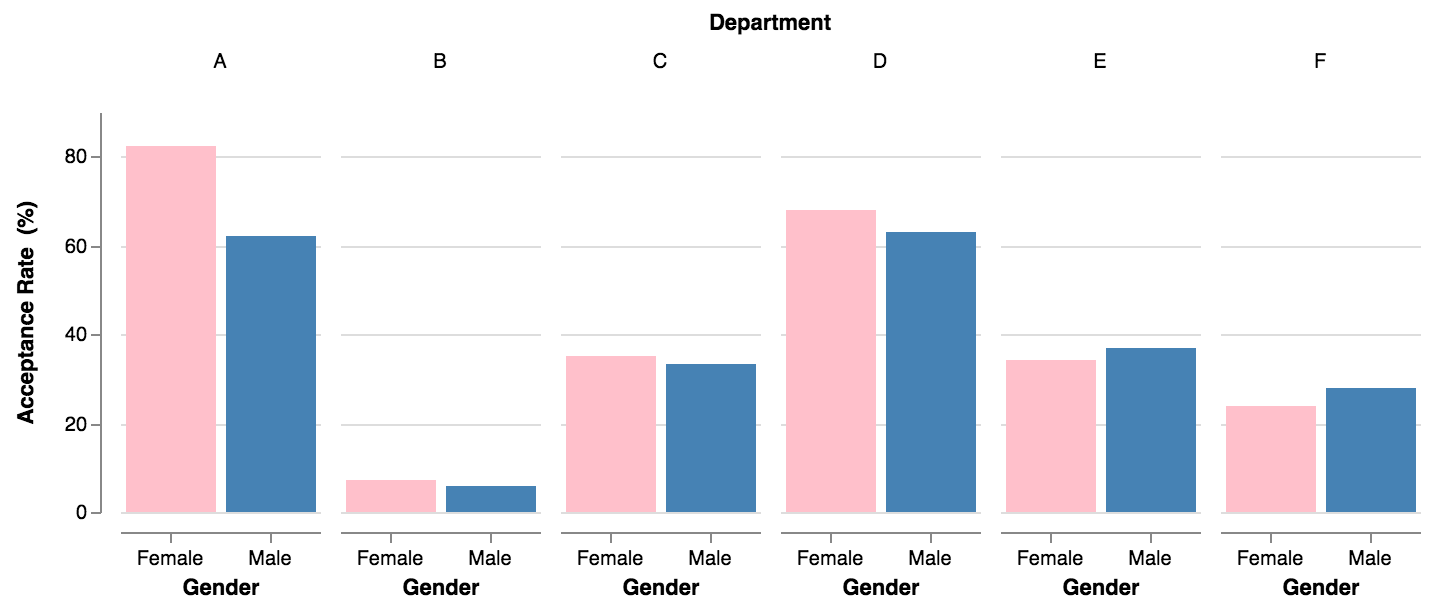
\includegraphics[width=\textwidth]{pictures/simpson2.png}
		\caption{Per-department acceptance rates, with a bias in favor of women in all but two departments.}
	\end{subfigure}
	\caption{Choices in how data are aggregated can completely alter the messages conveyed in visualizations. Here, the same data can produce bar charts with two seemingly opposite conclusions.}
	\label{fig:simpsons}
\end{figure}

\begin{figure*}
	\centering
	\begin{subfigure}{0.9\columnwidth}
		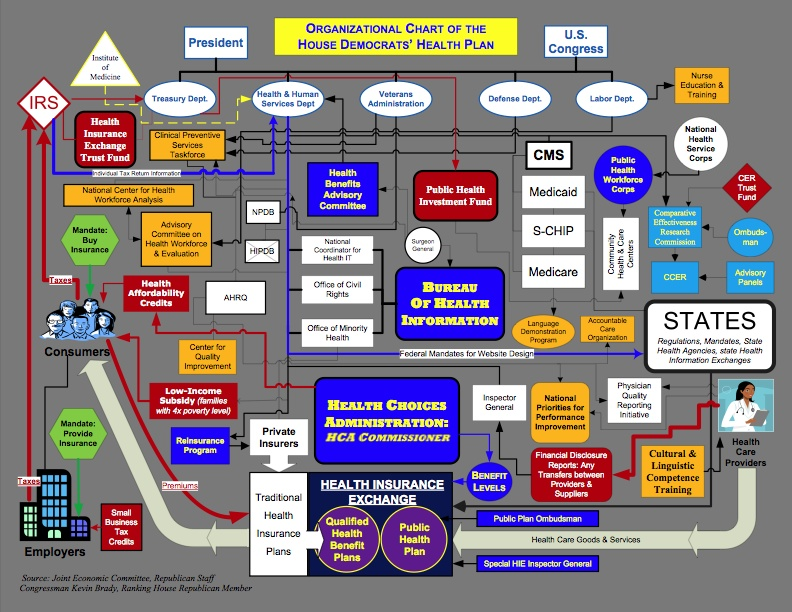
\includegraphics[width=\textwidth]{pictures/healthdirty.jpg}
		\caption{The original Republican flowchart of the ACA~\protect\cite{boehner}.}
	\end{subfigure}
	~
	\begin{subfigure}{0.9\columnwidth}
		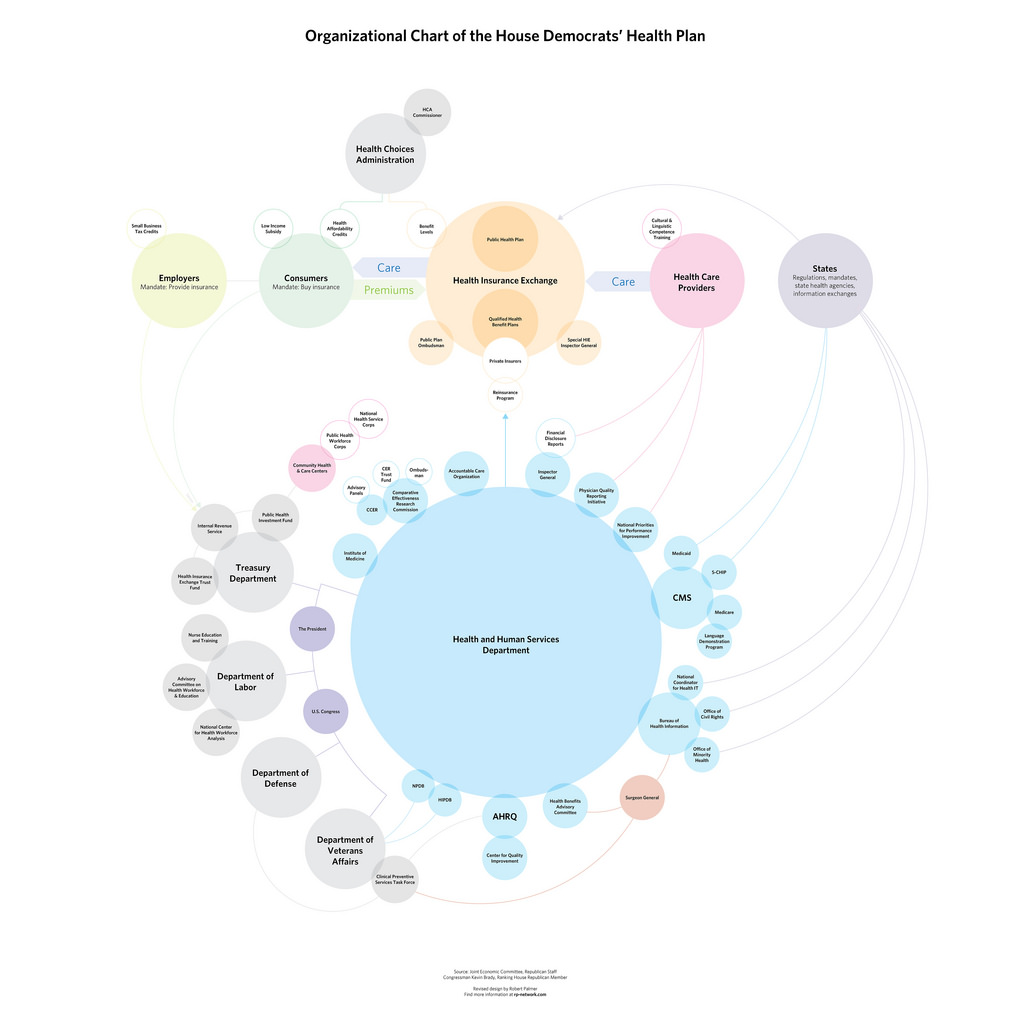
\includegraphics[width=\textwidth]{pictures/healthclean.jpg}
		\caption{Robert Palmer's cleaner version~\protect\cite{dontfuck}.}
	\end{subfigure}
	\caption{An example of intentional obfuscation in visualization design. Republicans in the U.S. House of Representatives produced a flowchart purporting to show the structure of the plan that would become the Affordable Care Act (ACA). Clashing colors, edge crossings, and busy fonts contribute to the impression that the plan is overly complex and impossible to understand. Robert Palmer, using the same topology information, produced a competing graphic titled ``Do not fuck with graphic designers'' as a passionate response to this intended obfuscation.}
	\label{fig:obfuscation}
\end{figure*}

If the attacker has full control over the data, then the potential for harm quite high. Similar to the non sequitur attacks above, the attacker can arbitrarily change the data and then make visualizations that faithfully present these false values. However, even if we presume that the individual data values are unaltered, there are still a number of ways that a designer can create harmful visualizations, by making malicious choices in how the data are aggregated, summarized, or filtered. Visualization designers are often given ``raw'' data, and are free to these choices themselves, and thus have a great deal of power over what messages a viewer can take away from the data.

Simpson's paradox is one example (Fig. \ref{fig:simpsons}) of this power. The same college admissions data can be used to show a bias either for or against women. This apparent contradiction is due to the fact that women were more likely to apply to departments with lower overall acceptance rates, and vice versa. By choosing how to aggregate and normalize the same data, the designer of the visualization can control the message of the chart. Presenting the full range of counts, percentages, and groups to circumvent these sorts of paradoxes requires visualizations more complex than simple histograms~\cite{poco2018extracting}. Data preparation choices related to aggregation and normalization, such as whether or not to discard outliers, or whether or not to smooth data, can also dramatically affect how data are visualized and subsequently interpreted.

\section{Obfuscation}

Another form of attack is to intentionally obscure the data values. That is, to make the process of visually extracting particular data values as arduous as possible. Even if the obfuscation does not make data illegible, a successful attack can make people less confident in the data, or their own understanding of the data. In some cases, presenting certain data as too complex to parse is a form of attack in and of itself (as in Fig~\ref{fig:obfuscation}).

Another attack which relies on obfuscation is to hide relevant information amongst a sea of less relevant or less damaging information. Dashboards and infographics often contain a dozen or more separate visualizations. If certain views or facets contain information contrary to the intended message of the attacker, then they can be placed in locations that require extra effort from the viewer to read (for instance, they require zooming, panning, or scrolling to encounter). Alternatively, black hat designers could attempt to counter solitary charts with damning information by including a large number of charts with supportive information. Even if the data in these supporting charts provides only weak or spurious evidence in support of the attacker's goal, their sheer number may mentally outweigh or exhaust the viewer (in argumentation, this technique is sometimes called a ``Gish Gallop''~\cite{gish}).

\begin{figure}
	\centering
	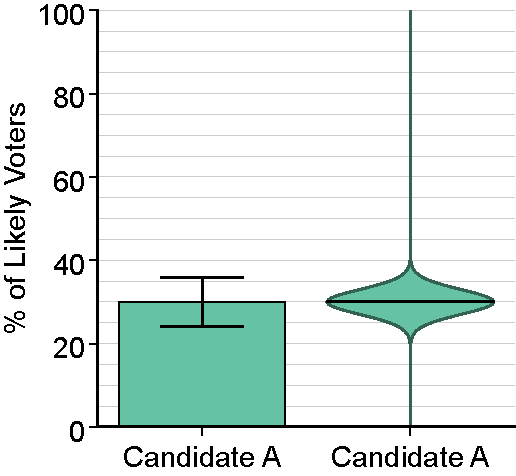
\includegraphics[width=0.45\columnwidth]{pictures/within}
	\caption{An example of a nudge, on polling data. The bars in bar charts create a visual metaphor of containment. This causes outcomes that would fall inside of the bar to perceived as liklier than values outside of the bar. Other visualizations lack this bias. In this sample polling data, viewers were more confident that Candidate A would underperform when presented with a bar chart (as on the left) than with a violin plot (as on the right)~\protect\cite{correll2014error}.}
	\label{fig:nudge}
\end{figure}

\section{Nudges}

The last form of attack we discuss is where the design of the visualization is altered to emphasize or de-emphasize certain patterns in the data. That is, the viewer is nudged toward or away from a particular interpretation of the data. These attacks are common in marketing; for instance, consumers are more likely to underestimate the price of goods when the price ends in $99$ rather than a round number (i.e., a product costing \$4.99 is more likely to be misremembered as costing less than a product costing \$5.00)~\cite{schindler1989effects}. However, these nudges are also present in visualizations. For instance, points in scatterplots are perceived as being more highly correlated when they are compressed in scale~\cite{cleveland1982variables}. Red glyphs in choropleth maps are perceived as having more area than green glyphs~\cite{cleveland1983color}. Points within the visual area of bars in bar charts are perceived as likelier than points outside of the bars~\cite{newman2012bar}. Estimates of y-intercepts in area charts are lower than in scatterplots~\cite{correll2017regression}. Attackers can take advantage of one or more of these nudges to systematically influence how data are perceived (as in Fig.~\ref{fig:nudge}). 

Although the impact of these individual nudges can be minor, these nudges could be compounded together for larger potential effects. Unlike the prior attack strategies, which can be easy for visualization experts to spot and correct, nudging can be subtle to identify, and (in some cases) even unavoidable. The interplay between visualization and decision-making is complex; minor tweaks in visual design can be sufficient for major changes in decision-making~\cite{inbar2007graphical}.

\section{Discussion}

As the collection and presentation of data becomes a larger part of peoples' lives, visualization becomes more and more important. This importance has a moral component: all powerful technologies have the potential for both use and abuse. We as a field should consider the full space of how visualizations can be misused. Performing this sort of analysis requires putting ourselves in the mindset of bad actors, and to consider the persuasive and rhetorical content of the visualizations that we make, even with the best of intentions~\cite{hullman2011visualization}. Enumerating these attacks offers the promise that we can detect them, and correct them where they are encountered.

There are three avenues of future work related to black hat vis. The first is taxonometric: we should enumerate the ways that visualizations can deceive or mislead. The examples presented in this paper, and in other works, are a fraction of this enormous space. The second avenue is empirical: rather than taking it on faith that these attacks are or are not effective to our target audiences, we should collect empirical evidence on the size and reliability of these effects (as per \cite{boy2017showing,pandey2014persuasive}). The last avenue is detection and prevention of bad behavior: ``white hat vis,'' using our analogy. There are many automated tools for generating and interacting with visualizations. To encourage the responsible use of these tools, we need to develop methods for detecting and correcting for their misuse. This ``defensive design'' could take the form of automated assistants (such as systems to detect and correct suboptimal color maps~\cite{poco2018extracting}), or could exist as codified design principles and best practices. However, at a minimum, we ought to bake in more supervision and guidance into visual analytics systems, through smart defaults, automated feedback, and explicit warnings to users and consumers of visualizations.
%% if specified like this the section will be committed in review mode
\acknowledgments{
This work was supported by a Moore Foundation Data-Driven Discovery Investigator award.
}

%\bibliographystyle{abbrv}
\bibliographystyle{abbrv-doi}
%\bibliographystyle{abbrv-doi-narrow}
%\bibliographystyle{abbrv-doi-hyperref}
%\bibliographystyle{abbrv-doi-hyperref-narrow}

\bibliography{decisive}
\end{document}
